\documentclass[]{article}

\usepackage{listings}
\usepackage{xcolor}
\usepackage{graphicx}
\usepackage[legalpaper, portrait, margin=1in]{geometry}

\definecolor{codegreen}{rgb}{0,0.6,0}
\definecolor{codegray}{rgb}{0.5,0.5,0.5}
\definecolor{codepurple}{rgb}{0.58,0,0.82}
\definecolor{backcolour}{rgb}{0.95,0.95,0.92}

\lstdefinestyle{codestyle}{
	backgroundcolor=\color{backcolour},
	commentstyle=\color{codegreen},
	keywordstyle=\color{magenta},
	numberstyle=\tiny\color{codegray},
	stringstyle=\color{codepurple},
	basicstyle=\ttfamily\footnotesize,
	breakatwhitespace=false,
	breaklines=true,
	captionpos=b,
	keepspaces=true,
	numbers=left,
	numbersep=5pt,
	showspaces=false,
	showstringspaces=false,
	showtabs=false,
	tabsize=2,
}

\lstset{style=codestyle}
% Title Page
\title{Operating System Simulation implementing Multi-level Priority Queue with Round-robin scheduling and Segmented Paging memory management system}
\author{Tran Trung Nguyen - 2052196 \\
Nguyen Xuan Bach - 2052196}
\date{\today}

\begin{document}
\maketitle

\newpage
\tableofcontents
\newpage

\section{Introduction}
This report will summarize the theories and implementation details of a working OS\textit{(Operating System)} simulation written in C++, which implements a system of \textbf{Multi-Level Priority Queue} scheduler and also a \textbf{Segmentation with Paging} memory management module.
\section{Implementation}
\subsection{Scheduler}
\subsubsection{Explanation}
A \textbf{Multi-Level Priority Queue} or \textbf{MLpQ} consists of multiple queues, representing multiple levels of priorities. Processes sitting in higher level queues will be executed first. Because \textit{priority queues} are used, in each level, added processes will also be queued-up based on their priority with respect to other existing processes.
\\
Note that these two priority index are different.\\
\\
Usually, each level of MLQ stores a type of process, representing their importantness. For example:
\begin{itemize}
	\item \textbf{Highest priority} - System processes, goes to \textbf{Queue 1}
	\item \textbf{High priority} - Interactive processes, goes to \textbf{Queue 2}
	\item \textbf{Lowest priority} - Batch processes, goes to \textbf{Queue 3}
\end{itemize}
and processes of each level will be stored in ready queues based on their priority with respect to other processes in the same level. For example, in level 3 \textbf{(Queue 3)} of batch processes:
\begin{figure}[h]
	\caption{In the same level, processes are organized such that processes with higher \lstinline|priority| is closer to the top}
	\centering
	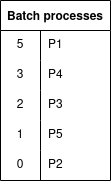
\includegraphics[width=0.15\textwidth]{content/queue_priority.png}
\end{figure}
\\
\begin{figure}[h]
	\caption{A time-sequence diagram of processes scheduled with MLqQ and round-robin policy for all levels}
	\centering
	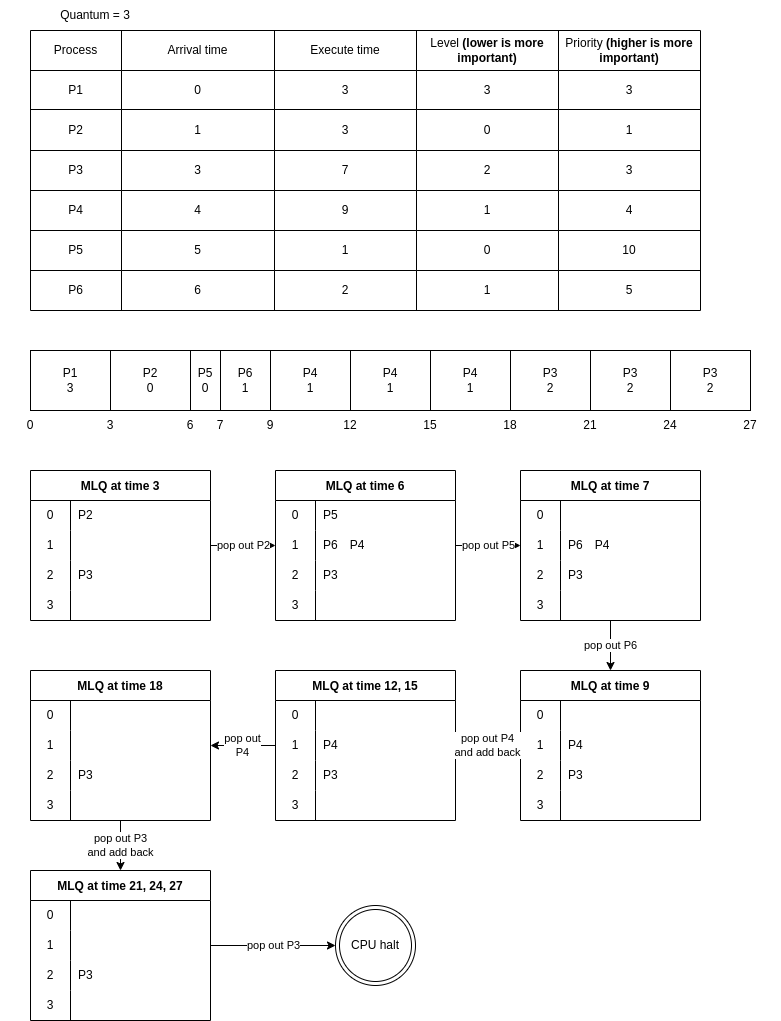
\includegraphics[height=0.5\textheight]{content/mlq_diagram.png}
\end{figure}
A process can be represented in code as such that it can be used with a MLQ:
\begin{lstlisting}[language=C++]
/* PCB, describe information about a process */
struct pcb_t {
	uint32_t pid;    /* Process ID */
	uint32_t priority; /* Task with higher priority runs first */
	uint32_t prio; /* Higher prio lives in higher queue level */
		
	/* Other properties */
		
	/* Constructor */
};
\end{lstlisting}
\newpage
\subsubsection{Priority queue}
A \textbf{priority queue} is a modified version of a queue where elements are organized with respect to their priority. By that principle, the priority of a process is designated through its property \textbf{priority}. Processes of highest priority is put to the top and lowest is put to the bottom. \\
\\
C++ implementation of a priority queue can be found in \lstinline|<queue>| library.
\begin{lstlisting}[language=C++]
class queue_t {
private:
	/* 
	 * Priority queue is based on a max_heap
	 * First parameter specifies the data type stored in the queue
	 * Second specifies which implementation of a list is used
	 * Last specifies a comparator, which compares 2 processes 
	*/
	std::priority_queue<std::shared_ptr<pcb_t>, std::vector<std::shared_ptr<pcb_t>>, pcb_comparator> q;
#ifdef OPTIMIZED_SCH
	/* Reserved for an optimized version of MLQ */
#endif
public:
	/* Add new process to queue */
	void enqueue(std::shared_ptr<pcb_t> proc);
		
	/* Dequeue the top priority process */
	std::shared_ptr<pcb_t> dequeue();
		
	/* Check if queue is empty */
	bool empty();
};
\end{lstlisting}
Processes are compared by implementing a comparator class - in this case, \lstinline|pcb_comparator|. Processes with lower \lstinline|priority| is prioritized over higher ones and are put at the closer to the top of the queue.
\begin{lstlisting}[language=C++]
/* Define necessary methods to compare the priority between processes */
class pcb_comparator {
	public:
	bool operator()(std::shared_ptr<pcb_t> const &a, std::shared_ptr<pcb_t> const &b) {
		return (a->priority < b->priority);
	}
};
\end{lstlisting}
The class \lstinline|queue_t| is implemented as such:
\begin{lstlisting}[language=C++]
void queue_t::enqueue(std::shared_ptr<pcb_t> proc) {
	/* Enqueue new process */
	if (q.size() == MAX_QUEUE_SIZE) {
		perror("Queue overflow while enqueue-ing\n");
		return;
	}
	q.push(proc);
}

std::shared_ptr<pcb_t> queue_t::dequeue() {
	/* Returns the process of highest priority */
	if (empty()) {
		perror("Dequeue-ing from empty queue\n");
		return nullptr;
	}
	std::shared_ptr<pcb_t> top = q.top();
	q.pop();
	return top;
}

bool queue_t::empty() {
	return q.empty();
}
\end{lstlisting}
\subsubsection{Scheduling algorithm}
The scheduler is put into a single class. Objects of this class will include an array of priority queues, which was explained earlier, and a lock, to avoid race conditions, since there will be multiple threads using the same scheduler at the same time.
\begin{lstlisting}[language=C++]
#define MAX_PRIO 512

class mlq_scheduler_t {
private:
	queue_t m_q_Ready[MAX_PRIO];
#ifdef OPTIMIZED_SCH
	/* Reserved for optimized version of MLQ */
#endif
	std::mutex m_Lock;
public:
	/* Extract processes from the priority queue */
	std::shared_ptr<pcb_t> get_proc();
	
	/* Add process to MLQ scheduler */
	void add_proc(const std::shared_ptr<pcb_t> &proc);
};
\end{lstlisting}
\lstinline|add_proc| simply adds the given process in the correct queue, determined based on its \lstinline|prio| property. However, different from the way priority queues organize its processes based on the \lstinline|priority| property, processes with lower \lstinline|prio| will be put into queue of higher level.
\begin{lstlisting}[language=C++]
void mlq_scheduler_t::add_proc(const std::shared_ptr<pcb_t> &proc) {
	std::unique_lock lock(m_Lock);
	/* O(log n) */
	m_q_Ready[(MAX_PRIO - 1) - proc->prio].enqueue(proc);
#ifdef OPTIMIZED_SCH
	/* Reserved for optimized version of MLQ
#endif
}
\end{lstlisting}
\lstinline|get_proc| is also simple to understand. It is used by the CPU to retrieve a process after each quantum finishes. It goes through the array of queues, from top \textbf{(highest priority)} to bottom, if it sees a non-empty queue, it takes the top priority process from that queue then stops and feeds that process back to the CPU. This ensures that the top prioritized processes always get executed first.
\begin{lstlisting}[language=C++]
std::shared_ptr<pcb_t> mlq_scheduler_t::get_proc() {
	std::unique_lock lock(m_Lock);
#ifdef OPTIMIZED_SCH
	/* Reserved for optimized version of MLQ */
#else
	/* Naive approach */
	/* O(MAX_PRIO) */
	for (uint32_t i = 0; i < MAX_PRIO; i += 1) {
		if (!m_q_Ready[i].empty()) {
			return m_q_Ready[i].dequeue();
		}
	}
#endif
	return nullptr;
}
\end{lstlisting}
However, this algorithm can be optimized \textbf{(in term of speed)}. With the naive approach, it retrieve the process the CPU at a worst-case complexity of \textbf{MAX\_PRIO*O(MAX\_PRIO)}, when all of the process are living in the lowest queue. CPU goes through the queues every cycle just to discover it does not have any process queuing up at all.
At a tradeoff of adding another priority queue, we can reduce this algorithm to a worst-case of $O(log n)$ where \textbf{n} is the number of process at any given time inside the MLQ.
\\
Whenever \lstinline|add_proc| is called, the optimized algorithm adds an entry of the \lstinline|prio| of the newly added process inside a priority queue.
\begin{lstlisting}[language=C++]
class mlq_scheduler_t {
private:
	queue_t m_q_Ready[MAX_PRIO];
#ifdef OPTIMIZED_SCH
	std::priority_queue<uint32_t, std::vector<uint32_t>, std::greater<>> m_q_Access;
#endif
	std::mutex m_Lock;
public:
	/* Methods */
};
\end{lstlisting}
\begin{lstlisting}[language=C++]
void mlq_scheduler_t::add_proc(const std::shared_ptr<pcb_t> &proc) {
	std::unique_lock lock(m_Lock);
	/* O(log n) */
	m_q_Ready[(MAX_PRIO - 1) - proc->prio].enqueue(proc);
#ifdef OPTIMIZED_SCH
	/* O(log n) */
	m_q_Access.push(proc->prio);
#endif
}
\end{lstlisting}
Next time \lstinline|get_proc| is called, it takes out the top element of that queue, which is the index where the top prioritized process lives inside the MLQ.
\begin{lstlisting}[language=C++]
std::shared_ptr<pcb_t> mlq_scheduler_t::get_proc() {
	std::unique_lock lock(m_Lock);
#ifdef OPTIMIZED_SCH
	/* O(1) */
	if (!m_q_Access.empty()) {
		uint32_t prioritized_next_level = m_q_Access.top();
		/* O(log n) : n is the number of processes */
		m_q_Access.pop();
		/* O(1) */
		if (!m_q_Ready[MAX_PRIO - prioritized_next_level].empty()) {
			/* O(log n) : n is the size of this level queue */
			return m_q_Ready[MAX_PRIO - prioritized_next_level].dequeue();
		}
	}
#else
	/* Naive approach */	
#endif
	return nullptr;
}
\end{lstlisting}
Overall, this approach takes a bit more storage to store the newly added queue.\\
\\
\lstinline|uint32_t| generally have an allocated size of 4 byte, at any given point of 10000 process, it consumes 40KB more than the naive approach, where as the naive approach complexity might just be $O(log 10000)$ \textbf{(all the processes are living in the top queue)} or $O(9999*log 10000)$ \textbf{(all of the processes are living in the bottom queue)}. The optimized scheduler retrieve the process at $O(log 10000)$ for all of the non-best cases where the MLQ is not empty \textbf{(in that case, the complexity is $O(1)$)}.\\
\\
\lstinline|add_proc| will have a higher complexity as well. However, it is used much less heavily than \lstinline|get_proc|. Therefore, the tradeoff is worth it.

\newpage
\subsection{Memory management}
For memory management, \textbf{Segmented Paging} is used.
\subsubsection{Theory}
The memory management module specifies locations to the CPU through a virtual address space. To the CPU, it appears that the allocated memory region is contiguous and treat it as such. However, under the hood, the might be some translation of that virtual address into physical address, which is the address pointing to the actual location of storage on the physical memory.\\
\\
The translation of virtual address is based on how memory allocation is done the module, and there are a few methods to do so.
\paragraph{Paging}
\textbf{Paging} means to seperate the physical memory into small chunks - often called \textit{frames}. The virtual address space is also split into equally sized chunks - called \textit{pages}. A page maps to a frame and they are equal in size, meaning that a space of 1 byte in a virtual address space is equivalent to 1 byte in the physical memory. A process memory is assigned in unit of pages. It appears to the CPU that memory is contigious.\\
\\
However, frames associated to those pages might not always be next to each other on the physical memory. Using a page table, the management module knows which page and frames are associated to each other, so it does not matter where the frames are. In this way, physical memory does not need to be contiguous and thus eliminate the possibility of \textbf{external fragmentation}.
\begin{figure}[h]
	\caption{Implementation of paging}
	\centering
	\vspace*{5mm}
	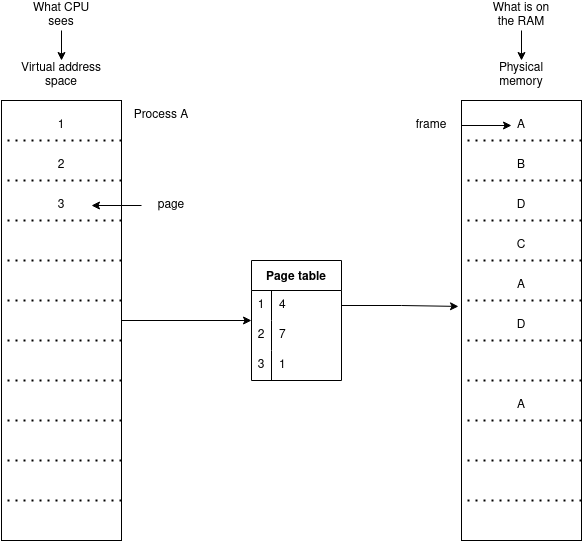
\includegraphics[width=0.5\textwidth]{content/paging.png}
\end{figure}
\paragraph{Segmentation}
Instead of seperating physical memory into frames, \textbf{segmentation} split the process into smaller portions - called \textit{segments}. Each segments gets its own parts in the virtual address space. The segments varies in size and are mapped to the physical memory using a \textit{segmentation table}, which stores the beginning physical address and the length of the storage for each segments. \\
\\
However, it suffers from external fragmentation, when memory are still allocated in smaller - but also not so small chunks, just when needed.
\newpage
\begin{figure}[h]
	\caption{Implementation of segmentation, which does not avoid external fragmentation}
	\centering
	\vspace*{5mm}
	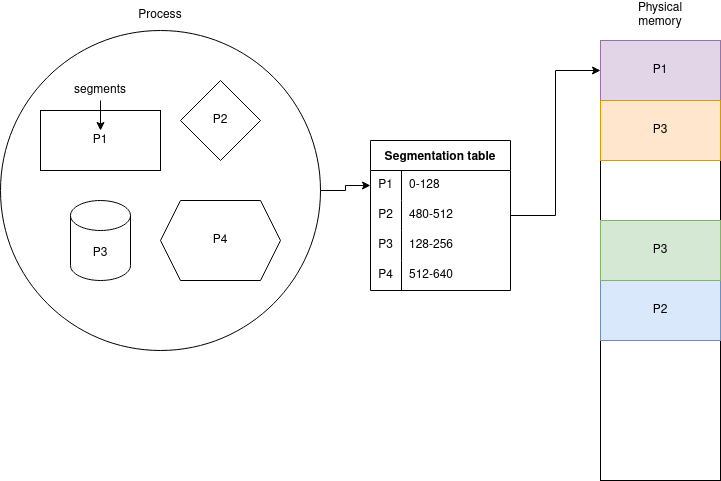
\includegraphics[width=0.5\textwidth]{content/segmentation.png}
\end{figure}
\paragraph{Segmented paging}
\subparagraph{Disadvantage of single-level paging}
If the virtual address space is large, then the page table may takes up a lot of space in the main memory.\\
For example, a 4KB page requires 12 bits ($2^{12}$) for its offset. A 32-bit virtual address space can hold upto $2^{32} / 2^{12} = 2^{20}$ number of pages. A page table takes up 2.5MB in the memory ($20 bits *2^{20}$). Since each process owns a page table, this amounts to a lot of memory being used for paging. For a system of a 64-bit virtual address page, a single page table cannot even fits in the physical memory.
\subparagraph{What is segmented paging}
In segmented paging, the physical memory is segmented, and each segments is split into pages. This saves a lot of space, due to indexing of pages takes much less bits. \textit{Segmented paging} means to divide the virtual address space into segments and divide each segments into pages
\subsubsection{Implementation}
\paragraph{Allocation}
A process needs registers to stores its memory regions virtual address. 
\begin{lstlisting}[language=C++]
/* PCB, describe information about a process */
struct pcb_t {
	uint32_t pid;    /* Process ID */
	code_seg_t code;    /* Code segment, simulated as the actual tasks */
	
	addr_t regs[10]{}; /* Registers, store address of allocated regions */
					   /* Stores virtual addresses */
	
	uint32_t pc{}; /* Program counter, pointing to next instruction */
	uint32_t bp{PAGE_SIZE};    /* Break pointer */
	
	page_table_t seg_table; /* Page table, will be explained in depth later */

	/* Other */
	
	/* Constructor */
};
\end{lstlisting}
These are the structures of the segmentation tables and page tables.
\begin{lstlisting}[language=C++]
/* Second layer */
struct trans_table_entry_t {
	addr_t v_index; // The index of virtual address
	addr_t p_index; // The index of physical address
};

struct trans_table_t {
	/* A row in the page table of the second layer */
	trans_table_entry_t table[1 << SECOND_LV_LEN];
	int size;
};

/* Mapping virtual addresses and physical ones */
struct page_table_entry_t {
	addr_t v_index{};    // Virtual index
	std::shared_ptr<trans_table_t> pages{};
};

struct page_table_t {
	/* Translation table for the first layer */
	std::vector<page_table_entry_t> table;
	
	page_table_t() : table(1 << FIRST_LV_LEN) {}
};
\end{lstlisting}
On allocation, the management module is given the allocation size. First it uses the \lstinline|mem_stat| list, which tracks used frames to determine if the size can be allocated sufficiently.
\begin{lstlisting}[language=C++]
addr_t memory_t::alloc_mem(uint32_t size, pcb_t *proc) {
	std::unique_lock<std::mutex> lock(m_Lock);
	addr_t ret_mem = 0;
	/* Allocate [size] byte in the memory for the
	* process [proc] and save the address of the first
	* byte in the allocated memory region to [ret_mem].
	*/
	
	/* Calculate the number pages required to host the requested memory */
	//uint32_t num_pages = (size % PAGE_SIZE) ? size / PAGE_SIZE :
	//size / PAGE_SIZE + 1; // Number of pages we will use
	
	uint32_t num_pages = (size + PAGE_SIZE - 1) / PAGE_SIZE;
	int mem_avail = 0; // We could allocate new memory region or not?
	
	/* First we must check if the amount of free memory in
	* virtual address space and physical address space is
	* large enough to represent the amount of required memory
	*
	* If so, set 1 to [mem_avail].
	*/
	
	uint32_t available_pages = 0;
	for (int i = 0; i < NUM_PAGES; i += 1) {
		if (_mem_stat[i].proc <= 0) {
			/* Not allocated */
			available_pages += 1;
		}
		if (available_pages >= num_pages) {
			break;
		}
	}
	/* Check if new memory region can be allocated
	*
	* On the physical address space, the number of pages must not be less than number of available pages
	* As for virtual address space, the size span from the breakpoint to its final segment must be less than the maximum address possible
	* (not more than 20 bits)
	*/
	if (available_pages >= num_pages) {
		if (proc->bp + (num_pages * PAGE_SIZE) <= RAM_SIZE) {
			mem_avail = 1;
		}
	}
	
	
	if (mem_avail) {
		/* Allocation */
	}
	return ret_mem;
}
\end{lstlisting}
It then allocates the memory according to the given size. For every new page added, it proceed to find an unused frame, then continue to add the index of that frame into the corresponding segmentation table and page table tracking the newly added page, found by extracting the first 5 bits and second 5 bits of its virtual address, respectively.\\
\\
After, it updates the \lstinline|mem_stat|.
\begin{lstlisting}[language=C++]
if (mem_avail) {
	/* We could allocate new memory region to the process */
	ret_mem = proc->bp;
	proc->bp += num_pages * PAGE_SIZE;
	/* Update status of physical pages which will be allocated
	* to [proc] in _mem_stat. Tasks to do:
	* 	- Update [proc], [index], and [next] field
	* 	- Add entries to segment table page tables of [proc]
	* 	  to ensure accesses to allocated memory slot is
	* 	  valid. */
	for (long phys_index = 0,
	page_index = 0,
	prev_index = -1;; phys_index += 1) {
		if (_mem_stat[phys_index].proc > 0) {
			/* Allocated, skip */
			continue;
		}
		
		/* Update the segment table */
		/* Calculate the virtual address */
		addr_t v_addr = ret_mem + (page_index * PAGE_SIZE);
		// printf("Virtual address: %d\n", v_addr);
		
		addr_t first_level_index = get_first_lv(v_addr);
		addr_t second_level_index = get_second_lv(v_addr);
		
		/* Update the level 1 segment */
		auto &first_level_entry = proc->seg_table.table.at(first_level_index);
		if (first_level_entry.v_index == 0) {
			first_level_entry.v_index = 1;
			first_level_entry.pages = std::make_shared<trans_table_t>();
		}
		
		/* Update the level 2 segment */
		auto &second_level_entry = first_level_entry.pages->table[second_level_index];
		second_level_entry.v_index = 1;
		second_level_entry.p_index = (addr_t) phys_index;
		first_level_entry.pages->size += 1;
		
		/* Update the memory status */
		if (prev_index >= 0) {
			/* May cause problem by casting to int */
			/* Phys index have type uint32_t with max value greater than int in _mem_stat
			* However, ->next of the last page must be -1
			* _mem_state entries will be long
			*/
			_mem_stat[prev_index].next = phys_index;
		}
		prev_index = phys_index;
		
		_mem_stat[phys_index].proc = proc->pid;
		_mem_stat[phys_index].index = page_index;
		
		page_index += 1;
		if (page_index >= num_pages) {
			/* Last page has next of (-1) */
			_mem_stat[phys_index].next = -1;
			break;
		}
	}
}
\end{lstlisting}
\paragraph{Deallocation}
On deallocation using \lstinline|free_mem|, the virtual address is provided. The management module can then translate that virtual address into the physical address, or in this simulation, the index of the allocated frames in \lstinline|mem_stat|.\\
\\
The translation includes extracting the first 5 bits to find the segmentation table, second 5 bits to find the page table, which stores the \lstinline|p_index| that the virtual address is representing, then return a physical address, which is a combination of 20 bits, including the first 10 bits, representing the \lstinline|p_index| found earlier (\lstinline|MAX_PAGES| is $2^{10}$ pages) and last 10 bits representing the page offset, extracted from the virtual address provided.
\begin{lstlisting}[language=C++]
/* Translate virtual address to physical address */
addr_t memory_t::translate(addr_t virtual_addr, pcb_t *proc) {
	/* Offset of the virtual address */
	addr_t offset = get_offset(virtual_addr);
	
	/* The first layer index */
	addr_t first_lv = get_first_lv(virtual_addr);
	
	/* The second layer index */
	addr_t second_lv = get_second_lv(virtual_addr);
	/*
	* Example: 13535
	* 00000|01101|0011011111
	*
	
	/* Search in the first level */
	std::shared_ptr<trans_table_t> trans_table = proc->seg_table.table[first_lv].pages;
	if (proc->seg_table.table[first_lv].v_index) {
		if (trans_table->table[second_lv].v_index) {
			/* Concatenate the offset of the virtual addess
			* to [p_index] field of trans_table->table
			*/
			
			/*
			* offset   = 0000000000|1100110101
			* addr     = 1111111111|1111111111
			* [...]    = 1111111111|1100110101
			*/
			
			/* Shift left by OFFSET_LEN (in this case is 10) then perform bitwise OR with offset
			* to concatenate page offset provided by the virtual address
			*/
			return (trans_table->table[second_lv].p_index << OFFSET_LEN | offset);
		}
	}
	
	/* uint32_t has more number needed for indexing in this exercise */
	return INT32_MAX;
}
\end{lstlisting}
Deallocation then happens easily with the provided physical address. It works by finding all pages starting from the virtual address \lstinline|address| supplied by the instruction, then attempt to clear all of its page table, then segment table, then free up the pages by resetting \lstinline|mem_stat| at the physical address got through translation.
\begin{lstlisting}[language=C++]
int memory_t::free_mem(addr_t address, pcb_t *proc) {
	std::unique_lock<std::mutex> lock(m_Lock);
	/* Release memory region allocated by [proc]. The first byte of
	* this region is indicated by [address]
	* 	- Set flag [proc] of physical page use by the memory block
	* 	  back to zero to indicate that it is free.
	* 	- Remove unused entries in segment table and page tables of
	* 	  the process [proc].
	* 	- Remember to use lock to protect the memory from other
	* 	  processes.  */
	addr_t physical_addr = translate(address, proc);
	if (physical_addr == INT32_MAX) {
		return 1;
	}
	
	addr_t physical_start = physical_addr >> OFFSET_LEN;
	for (long physical_index = physical_start,
	page_index = 0;
	physical_index != -1; page_index += 1) {
		addr_t virtual_addr = address + (page_index * PAGE_SIZE);
		addr_t first_level_index = get_first_lv(virtual_addr);
		addr_t second_level_index = get_second_lv(virtual_addr);
		
		/* Clean second level */
		auto &trans_table = proc->seg_table.table[first_level_index].pages;
		trans_table->table[second_level_index].v_index = 0;
		trans_table->size -= 1;
		
		/* Clean first level */
		if (trans_table->size == 0) {
			auto &page_table = proc->seg_table.table;
			page_table[first_level_index].pages.reset();
			page_table[first_level_index].v_index = 0;
		}
		
		/* Move to next mem_stat and clear */
		_mem_stat[physical_index].proc = 0;
		physical_index = _mem_stat[physical_index].next;
	}
	return 0;
}
\end{lstlisting}
\paragraph{Write \& Read}
As frames are allocated by storing the \lstinline|p_index| (index of the allocated frames) in the appropriate segmentation table and page index, memory can be written into those frames as such:
\begin{lstlisting}[language=C++]
int memory_t::read_mem(addr_t address, pcb_t *proc, BYTE *data) {
	addr_t physical_addr = translate(address, proc);
	if (physical_addr != INT32_MAX) {
		*data = _ram[physical_addr];
		return 0;
	} else {
		return 1;
	}
}

int memory_t::write_mem(addr_t address, pcb_t *proc, BYTE data) {
	addr_t physical_addr = translate(address, proc);
	// printf("At: %d\n", physical_addr);
	// printf("Data -> memory: %d\n", data);
	if (physical_addr != INT32_MAX) {
		_ram[physical_addr] = data;
		return 0;
	} else {
		return 1;
	}
}
\end{lstlisting}
As mentioned earlier, the physical address in this case is a combination of \lstinline|p_index| (which frame to write to) and the offset (where inside that frame) supplied by the \lstinline|read| and \lstinline|write| instruction.
\subsubsection{Example}
This section will show an example of how the allocation algorithm work when allocating and deallocating memory.
\paragraph{Allocation}
The allocation takes in a size and the index of the register inside the process where the virtual address for this memory region is stored.
\begin{lstlisting}
alloc 13535 0
\end{lstlisting}
To inspect the result, the \lstinline|dump| method of the management module is used. It goes through the \lstinline|mem_stat| and print out the list of frames allocated to host this memory size. After the dumping, the result of the allocation is:
\begin{lstlisting}
000: 0-1023 - PID: 01 (idx 000, nxt: 001)
001: 1024-2047 - PID: 01 (idx 001, nxt: 002)
002: 2048-3071 - PID: 01 (idx 002, nxt: 003)
003: 3072-4095 - PID: 01 (idx 003, nxt: 004)
004: 4096-5119 - PID: 01 (idx 004, nxt: 005)
005: 5120-6143 - PID: 01 (idx 005, nxt: 006)
006: 6144-7167 - PID: 01 (idx 006, nxt: 007)
007: 7168-8191 - PID: 01 (idx 007, nxt: 008)
008: 8192-9215 - PID: 01 (idx 008, nxt: 009)
009: 9216-10239 - PID: 01 (idx 009, nxt: 010)
010: 10240-11263 - PID: 01 (idx 010, nxt: 011)
011: 11264-12287 - PID: 01 (idx 011, nxt: 012)
012: 12288-13311 - PID: 01 (idx 012, nxt: 013)
013: 13312-14335 - PID: 01 (idx 013, nxt: -01)
\end{lstlisting}
There were in total of 14 frames being allocated for this process. Since the default \lstinline|PAGE_SIZE| is 1024 bits or 1 byte, 14 frames were equals to $14*1024=14336$ bits of memory, or 14 bytes, which is the right amount of memory being supplied. \\
\\
This number might seems a little higher than the amount that was requested. However, this is due to \textbf{internal fragmentation}, which is expected. Memory is split into blocks of 1024 bits but 13535 can not be divided perfectly to 1024 (bits), resulting to a block, being allocated to host a lower amount of memory than its capacity.\\
\\
Let's allocate a another memory region:
\begin{lstlisting}
alloc 13535 0
alloc 1568 1
\end{lstlisting}
\paragraph{Deallocation}
This region virtual address is stored inside the register of index 1. The expected behavior is that the management module will allocate 2 more frames to host is memory ($1568 / 1024$).
\begin{lstlisting}
...
013: 13312-14335 - PID: 01 (idx 013, nxt: -01)
014: 14336-15359 - PID: 01 (idx 000, nxt: 015)
015: 15360-16383 - PID: 01 (idx 001, nxt: -01)	
\end{lstlisting}
\lstinline|free| instruction can be used to free up the pages being used for next allocation. It required the register index used to specified. Let's free up the region that was allocated first.
 \begin{lstlisting}
alloc 13535 0
alloc 1568 1
free 0
\end{lstlisting}
The expected result is that the memory region stored in register 0 will be freed up, and the memory region in register 1 that was allocated earlier and not being touched will not be deallocate, as shown below.
\begin{lstlisting}
014: 14336-15359 - PID: 01 (idx 000, nxt: 015)
015: 15360-16383 - PID: 01 (idx 001, nxt: -01)
\end{lstlisting}
Now that frames from 001 to 013 are freed. During the next allocation, the new memory region will be allocated in a few of those frames.
\begin{lstlisting}[language=C++]
alloc 13535 0
alloc 1568 1
free 0
alloc 1386 2
\end{lstlisting}
\begin{lstlisting}
000: 0-1023 - PID: 01 (idx 000, nxt: 001)
001: 1024-2047 - PID: 01 (idx 001, nxt: -01)
014: 14336-15359 - PID: 01 (idx 000, nxt: 015)
015: 15360-16383 - PID: 01 (idx 001, nxt: -01)
\end{lstlisting}
\paragraph{Write \& Read}
Using the \lstinline|read| and \lstinline|write| instructions, data can be written into the frames. \lstinline|write| requires the data (write what), register index (which page) and offset (where inside the page)
\begin{lstlisting}
alloc 13535 0
alloc 1568 1
free 0
alloc 1386 2
write 10 1 20
write 21 2 1000
\end{lstlisting}
In the result below, \lstinline|003e8|(1000) is the offset provided by \lstinline|write| instruction given to the memory region at register 2. Since the allocated frames for that memory region lies from index 0-2047 as seen earlier, the instruction writes to memory in the first frame. Similarly for the \lstinline|write| instruction given to register 1, which writes to the $15^{th}$ frame.
\begin{lstlisting}
000: 0-1023 - PID: 01 (idx 000, nxt: 001)
003e8: 21
001: 1024-2047 - PID: 01 (idx 001, nxt: -01)
014: 14336-15359 - PID: 01 (idx 000, nxt: 015)
03814: 10
015: 15360-16383 - PID: 01 (idx 001, nxt: -01)
\end{lstlisting}
If the offset is increased for the \lstinline|write| instruction given to register 2, the data is written to the $1^{st}$ frame instead:
\begin{lstlisting}
alloc 13535 0
alloc 1568 1
free 0
alloc 1386 2
write 10 1 20
write 21 2 2000
\end{lstlisting}
\begin{lstlisting}
000: 0-1023 - PID: 01 (idx 000, nxt: 001)
001: 1024-2047 - PID: 01 (idx 001, nxt: -01)
007d0: 21
014: 14336-15359 - PID: 01 (idx 000, nxt: 015)
03814: 10
015: 15360-16383 - PID: 01 (idx 001, nxt: -01)
\end{lstlisting}
\section{Conclusion}
The simulation has presented a low-level designed of an \textit{operating system} incorporating MLQ \& Round-robin scheduling as well as a memory management module implementing segmented paging memory allocation system.
\end{document}          
